\section{Methodology}
\label{sec:methodology}

This section describes the proposed hybrid Transformer--CNN framework for multi-class oral disease classification from intraoral images. We first formulate the problem, followed by the overall architecture, feature extraction modules, data processing pipeline, training strategy, and evaluation metrics.

% ------------------------------------------------------------------
\subsection{Problem Formulation}
\label{subsec:problem_formulation}

Given an intraoral RGB image $I \in \mathbb{R}^{H \times W \times 3}$, the objective is to predict a disease class
$y \in \{0, 1, \ldots, C-1\}$, where $C=6$ denotes the number of oral disease categories. 
Each intraoral image is annotated with exactly one disease category, formulating the task as a multi-class classification problem.

The disease categories are summarized in Table~\ref{tab:diseases}.

\begin{table}[htbp]
\centering
\caption{Oral disease categories with clinical prevalence}
\label{tab:diseases}
\begin{tabular}{cll}
\toprule
\textbf{Index} & \textbf{Disease Category} & \textbf{Dataset \%} \\
\midrule
0 & Calculus & 10.11\% \\
1 & Caries & 18.58\% \\
2 & Gingivitis & 26.20\% \\
3 & Hypodontia & 10.97\% \\
4 & Tooth Discoloration & 14.31\% \\
5 & Ulcer & 19.83\% \\
\bottomrule
\end{tabular}
\end{table}

The multi-class formulation assumes mutual exclusivity between disease categories. The learning task is formulated as classifying each image into exactly one disease class, where the model outputs posterior probabilities $p_c = P(y = c \mid I)$ through softmax activation, with the predicted class being $\hat{y} = \arg\max_c p_c$.

% ------------------------------------------------------------------
\subsection{Proposed Hybrid Transformer--CNN Architecture}
\label{subsec:framework_architecture}

\subsubsection{Overall Architecture}

The proposed framework follows a hierarchical feature learning paradigm that integrates convolutional and Transformer-based representations, leveraging the complementary strengths of both architectures: CNNs excel at capturing local texture patterns and fine-grained details including lesion boundaries, and tooth surfaces. While Transformers model long-range spatial dependencies crucial for understanding disease co-occurrence patterns across the oral cavity.

The processing pipeline consists of the following stages:

\begin{enumerate}
    \item \textbf{Input}: Resized intraoral image of $224 \times 224 \times 3$
    \item \textbf{CNN Backbone}: Hierarchical extraction of local spatial features at multiple scales
    \item \textbf{Patch Embedding}: Conversion of CNN feature maps to token sequences
    \item \textbf{Transformer Encoder}: Window-based self-attention for global context modeling
    \item \textbf{Feature Fusion}: Multi-scale cross-attention between CNN and Transformer features
    \item \textbf{Classification Head}: Two-layer MLP with dropout and softmax activation
\end{enumerate}

Figure~\ref{fig:architecture} illustrates the complete architecture with feature dimensions at each stage.

\begin{figure}[htbp]
\centering
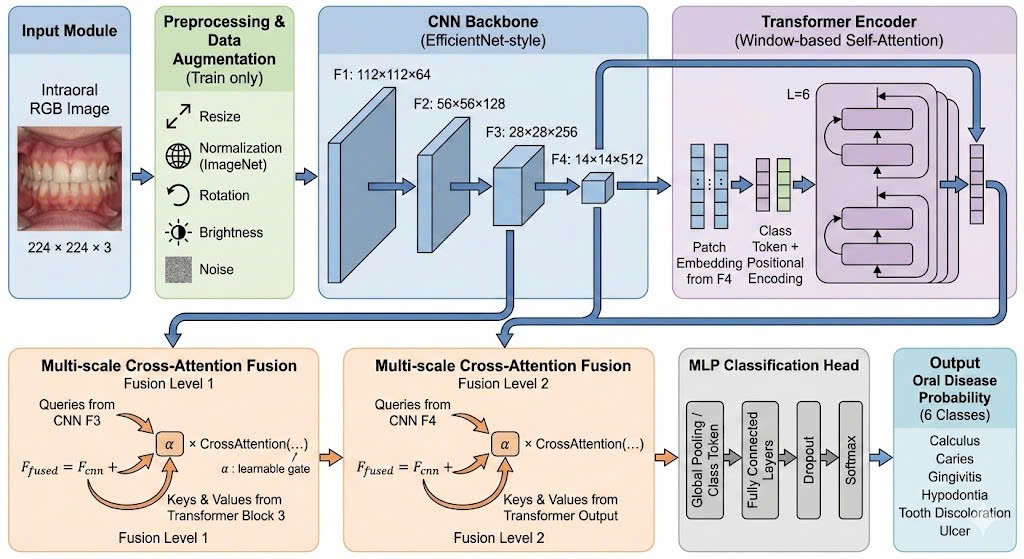
\includegraphics[width=\linewidth]{images/pipeline.png}
\caption{Hybrid Transformer--CNN architecture. The pipeline consists of: (1) Input Module receiving $224 \times 224 \times 3$ intraoral RGB images, (2) Preprocessing \& Data Augmentation including resize, normalization, rotation, brightness adjustment, and noise injection, (3) CNN Backbone (EfficientNet-style) extracting multi-scale features $\{\mathbf{F}_1, \mathbf{F}_2, \mathbf{F}_3, \mathbf{F}_4\}$ with channels $\{64, 128, 256, 512\}$, (4) Transformer Encoder with $L=6$ blocks of window-based self-attention, (5) Multi-scale Cross-Attention Fusion with learnable gate $\alpha$ at two levels, and (6) MLP Classification Head outputting probabilities for 6 oral disease classes.}
\label{fig:architecture}
\end{figure}

% ------------------------------------------------------------------
\subsubsection{CNN Backbone Networks}
\label{subsubsec:cnn_backbone}

To capture fine-grained local patterns such as lesion boundaries, calculus deposits, and enamel discoloration, the framework supports multiple pretrained CNN backbones initialized with ImageNet-1K weights. These networks offer different trade-offs between model capacity and computational complexity, as summarized in Table~\ref{tab:backbones}.
z
\begin{table}[htbp]
\centering
\caption{Supported CNN backbone networks with computational characteristics}
\label{tab:backbones}
\small
\begin{tabular}{llcc}
\toprule
\textbf{Model} & \textbf{Variants} & \textbf{Params} & \textbf{FLOPs (G)} \\
\midrule
MobileNetV3 & Small, Large & 1.5M--4.2M & 0.06--0.22 \\
EfficientNet & B0--B3 & 5.3M--12M & 0.39--1.8 \\
ResNet & 18, 34, 50 & 11.7M--25.6M & 1.8--4.1 \\
DenseNet & 121, 169 & 7.0M--14.1M & 2.8--3.4 \\
\bottomrule
\end{tabular}
\end{table}


For this study, we primarily adopt \textbf{EfficientNet-B0} as the default backbone due to its favorable accuracy-efficiency trade-off, achieving competitive performance with only 5.3M parameters. Ablation studies comparing different backbones are presented in Section~\ref{sec:ablation}.

Feature maps are extracted at four hierarchical stages with progressively increasing receptive fields:
\begin{itemize}
    \item \textbf{Stage 1} ($H/2 \times W/2 \times 64$): High-resolution features capturing fine details
    \item \textbf{Stage 2} ($H/4 \times W/4 \times 128$): Mid-level textures and patterns
    \item \textbf{Stage 3} ($H/8 \times W/8 \times 256$): Semantic features for lesion identification
    \item \textbf{Stage 4} ($H/16 \times W/16 \times 512$): High-level contextual representations
\end{itemize}

Features from stages 3 and 4 ($\mathbf{F}_3, \mathbf{F}_4$) are forwarded to the Transformer encoder, as they provide sufficient semantic abstraction while maintaining spatial resolution suitable for patch-based attention ($14 \times 14$ and $7 \times 7$ respectively).

% ------------------------------------------------------------------
\subsection{Transformer Encoder Module}
\label{subsec:transformer}

\subsubsection{Patch Embedding and Positional Encoding}

CNN feature maps from stage 4 ($\mathbf{F}_4 \in \mathbb{R}^{H/16 \times W/16 \times 512}$) are converted into a sequence of tokens. For an input of size $224 \times 224$, this produces a $14 \times 14$ spatial grid, which is flattened into $N = 196$ tokens.

Following ViT~\cite{dosovitskiy2021vit}, we prepend a learnable class token $\mathbf{t}_{\text{cls}}$ and add learnable positional embeddings $\mathbf{E}_{\text{pos}} \in \mathbb{R}^{(N+1) \times D}$ to inject spatial information:
\begin{equation}
\mathbf{Z}_0 = [\mathbf{t}_{\text{cls}}; \text{Flatten}(\mathbf{F}_4)] + \mathbf{E}_{\text{pos}},
\end{equation}
where $D$ is the embedding dimension (detailed in Table~\ref{tab:model_configs}).

\subsubsection{Window-Based Self-Attention}

To reduce the quadratic complexity of standard self-attention ($\mathcal{O}(N^2)$, which is prohibitive for high-resolution medical images), we adopt window-based self-attention inspired by Swin Transformer~\cite{liu2021swin}. The spatial tokens are partitioned into non-overlapping local windows of size $M \times M$, and self-attention is computed independently within each window.

Given query $Q$, key $K$, and value $V$ matrices for a window, attention is computed as:
\begin{equation}
\mathrm{Attention}(Q,K,V) =
\mathrm{softmax}\!\left(\frac{QK^\top}{\sqrt{d_k}} + B\right)V,
\end{equation}
where $d_k$ is the head dimension and $B \in \mathbb{R}^{M^2 \times M^2}$ is a learnable relative position bias matrix encoding spatial relationships within the window.

\textbf{Window size selection}: We use $M = 7$ following Swin Transformer design, which provides a favorable balance between local context (49 tokens per window) and computational efficiency. For our $14 \times 14$ feature maps, this creates $2 \times 2 = 4$ windows. The complexity is reduced from $\mathcal{O}((14 \times 14)^2) = \mathcal{O}(38{,}416)$ to $\mathcal{O}(4 \times 7^2 \times 7^2) = \mathcal{O}(9{,}604)$, achieving 4$\times$ efficiency gain.

\textbf{Multi-head attention}: Attention is computed in parallel across $h$ heads to capture diverse feature relationships:
\begin{equation}
\mathrm{MHSA}(\mathbf{Z}) = \mathrm{Concat}(\mathrm{head}_1, \dots, \mathrm{head}_h)W^O,
\end{equation}
where each head operates on a dimension of $d_k = D/h$. We use $h=8$ heads for the base model.

\subsubsection{Transformer Block}

Each Transformer block consists of window-based multi-head self-attention (W-MHSA) followed by a feed-forward network (FFN), both wrapped with residual connections and Layer Normalization (LN):

\begin{align}
\mathbf{Z}'_\ell &= \text{W-MHSA}(\text{LN}(\mathbf{Z}_{\ell-1})) + \mathbf{Z}_{\ell-1}, \\
\mathbf{Z}_\ell &= \text{FFN}(\text{LN}(\mathbf{Z}'_\ell)) + \mathbf{Z}'_\ell.
\end{align}

The FFN consists of two linear layers with GELU activation and expansion ratio 4:
\begin{equation}
\mathrm{FFN}(\mathbf{x}) = \mathrm{GELU}(\mathbf{x}W_1 + b_1)W_2 + b_2,
\end{equation}
where $W_1 \in \mathbb{R}^{D \times 4D}$ and $W_2 \in \mathbb{R}^{4D \times D}$.

\textbf{Architecture depth}: We stack $L$ Transformer blocks, where $L$ varies by model size (see Table~\ref{tab:model_configs}). The base model uses $L=6$ blocks, providing sufficient depth for global context modeling without overfitting on our dataset size ($\sim$9K training images).

\begin{table}[htbp]
\centering
\caption{Model configurations and hyperparameters}
\label{tab:model_configs}
\resizebox{0.48\textwidth}{!}{%
\begin{tabular}{lccc}
\toprule
\textbf{Hyperparameter} & \textbf{Small} & \textbf{Base} & \textbf{Large} \\
\midrule
Embedding dimension $D$ & 256 & 384 & 512 \\
Transformer blocks $L$ & 4 & 6 & 8 \\
Attention heads $h$ & 4 & 8 & 8 \\
Window size $M$ & 7 & 7 & 7 \\
FFN expansion ratio & 4 & 4 & 4 \\
Dropout rate & 0.1 & 0.3 & 0.3 \\
\midrule
Total parameters & 8.2M & 15.7M & 28.4M \\
FLOPs (G) & 1.2 & 2.8 & 5.1 \\
\bottomrule
\end{tabular}
}
\end{table}

\textbf{Design Contributions}: While our framework builds upon established components (window attention from Swin Transformer~\cite{liu2021swin}, cross-attention fusion mechanisms~\cite{chen2021transunet}), we introduce several adaptations specifically optimized for oral disease classification:
\begin{enumerate}
    \item \textbf{Learnable gated fusion ($\alpha$)}: Our gated residual connection (Eq.~\ref{eq:fusion}) with learnable $\alpha$ initialized to 0.1 allows the network to adaptively balance local CNN and global Transformer features during training, providing more flexibility than fixed-weight fusion approaches.
    \item \textbf{Multi-scale cross-attention}: We apply fusion at two scales (stages 3 and 4) rather than single-point fusion, enabling hierarchical feature integration.
    \item \textbf{Lightweight configuration}: Our base model achieves competitive performance with only 15.7M parameters---82\% smaller than ViT-Base (86M), 45\% smaller than Swin-Tiny (28.3M), and comparable to EfficientNet-B3 (12M) while incorporating global attention mechanisms absent in pure CNN architectures. This compact design enables deployment on standard clinical GPUs (8GB VRAM) with inference time <50ms per image.
\end{enumerate}

\subsubsection{Cross-Attention Feature Fusion}

To integrate local CNN features with global Transformer representations, we employ cross-attention fusion at multiple scales. Specifically, features from CNN stage 3 ($\mathbf{F}_3$) are fused with the output of Transformer block 3, and CNN stage 4 features ($\mathbf{F}_4$) are fused with the final Transformer output.

For each fusion point, CNN features serve as queries while Transformer features provide keys and values:
\begin{equation}
\mathrm{CrossAttn}(Q_{\text{cnn}}, K_{\text{trans}}, V_{\text{trans}})
=
\mathrm{softmax}\!\left(
\frac{Q_{\text{cnn}} K_{\text{trans}}^\top}{\sqrt{d_k}}
\right)
V_{\text{trans}}
\end{equation}



The fused features combine local and global information via a gated residual connection:
\begin{equation}
\mathbf{F}_{\text{fused}} =
\mathbf{F}_{\text{cnn}} + \alpha \cdot
\mathrm{CrossAttn}(Q_{\text{cnn}}, K_{\text{trans}}, V_{\text{trans}}),
\label{eq:fusion}
\end{equation}
where $\alpha$ is a learnable scaling parameter initialized to 0.1, allowing the network to gradually incorporate global context. This design is inspired by recent work showing that residual scaling improves training stability in hybrid architectures~\cite{touvron2021training}.

\textbf{Dimension alignment}: Before cross-attention, we project CNN and Transformer features to a common dimension $D$ using $1 \times 1$ convolutions for CNN features and linear layers for Transformer tokens.

% ------------------------------------------------------------------
\subsection{Data Processing Pipeline}
\label{subsec:data_pipeline}

\subsubsection{Data Augmentation}

To improve generalization and robustness to real-world imaging variations (different cameras, lighting, viewing angles), we apply extensive data augmentation during training. Augmentations are implemented using the \texttt{albumentations} library~\cite{albumentations} and applied with the following probabilities:

\begin{table*}[t]
\centering
\caption{Data augmentation strategy with application probabilities}
\label{tab:augmentation}
\small
\setlength{\tabcolsep}{6pt}
\begin{tabular}{p{5.2cm} p{7.5cm} c}
\toprule
\textbf{Augmentation} & \textbf{Parameters} & \textbf{Probability} \\
\midrule
\multicolumn{3}{l}{\textit{Geometric Transformations}} \\
Random Rotation & $\pm 15^\circ$ & 0.5 \\
Random Scaling & $0.8$--$1.2\times$ & 0.5 \\
Horizontal Flip & --- & 0.5 \\
ShiftScaleRotate & shift=$\pm10\%$, scale=$\pm10\%$ & 0.3 \\
Elastic Transform & $\alpha=50$, $\sigma=5$ & 0.2 \\
\midrule
\multicolumn{3}{l}{\textit{Photometric Augmentations}} \\
Brightness/Contrast & $\pm 20\%$ & 0.6 \\
Hue/Saturation & $\pm 10\%$ & 0.4 \\
Random Gamma & $\gamma \in [0.8, 1.2]$ & 0.3 \\
CLAHE & clip=2.0, tile=$8\times8$ & 0.3 \\
\midrule
\multicolumn{3}{l}{\textit{Noise and Occlusion}} \\
Gaussian Noise & $\sigma=0.01$ & 0.3 \\
Motion Blur & kernel=3--7 & 0.2 \\
CoarseDropout & holes=3--5, size=$16\times16$ & 0.3 \\
\bottomrule
\end{tabular}
\end{table*}



Augmentations are applied sequentially with independent random sampling. For validation and test sets, only resizing and normalization are applied to ensure unbiased evaluation.

\textbf{Design rationale}: Geometric augmentations simulate different viewing angles and patient positioning variability. Photometric augmentations address lighting inconsistencies common in clinical photography (natural vs. artificial light, flash vs. ambient). CoarseDropout encourages the model to learn from partial views, improving robustness to occlusions (tongue, saliva, dental tools).

\subsubsection{Class Imbalance Handling}

The dataset exhibits moderate class imbalance (2.6$\times$ ratio between most and least frequent classes, see Table~\ref{tab:diseases}). We address this through a three-pronged strategy:

\begin{enumerate}
\item \textbf{Stratified Splitting}: The pre-defined train/val/test splits maintain proportional class distributions, preventing evaluation bias.

\item \textbf{Class-Aware Weighted Sampling}: During training, we oversample minority classes using inverse frequency weighting. The sampling probability for class $c$ is:
\begin{equation}
w_c = \frac{N_{\text{total}}}{C \cdot N_c},
\end{equation}
where $N_{\text{total}} = 8{,}924$ is total training samples, $C=6$ is number of classes, and $N_c$ is samples in class $c$. This produces sampling weights: Calculus (1.60), Caries (0.87), Gingivitis (0.69), Hypodontia (1.54), Tooth Discoloration (1.13), Ulcer (0.82).

\item \textbf{Loss Function Weighting}: In addition to sampling, we apply class weights in the loss function (see Section~\ref{subsec:loss}).
\end{enumerate}

\textbf{Ablation}: Section~\ref{sec:ablation} compares this strategy against SMOTE oversampling and simple undersampling.

% ------------------------------------------------------------------
\subsection{Training Strategy}
\label{subsec:training}

\subsubsection{Loss Functions}
\label{subsec:loss}

For multi-class classification with imbalanced data, we investigate three loss functions designed to handle class imbalance and hard examples:

\textbf{1. Cross-Entropy (CE)} -- The standard multi-class loss:
\begin{equation}
\mathcal{L}_{\text{CE}} = -\log p_{y^*},
\end{equation}
where $y^* \in \{0, \ldots, C-1\}$ is the ground truth class and $p_{y^*}$ is the predicted probability for that class.

\textbf{2. Focal Loss}~\cite{lin2017focal} -- Down-weights well-classified examples to focus on hard cases:
\begin{equation}
\mathcal{L}_{\text{Focal}} = -(1-p_{y^*})^\gamma \log p_{y^*},
\end{equation}
with focusing parameter $\gamma=2$ (standard setting). This loss is particularly effective for addressing class imbalance by reducing the relative loss contribution from easy examples.

\textbf{3. Label Smoothing Cross-Entropy (LSCE)} -- Prevents overconfidence and improves calibration:
\begin{equation}
\mathcal{L}_{\text{LSCE}} = (1-\epsilon)\mathcal{L}_{\text{CE}} + \frac{\epsilon}{C}\sum_{c=1}^{C} (-\log p_c),
\end{equation}
with smoothing parameter $\epsilon = 0.1$. This distributes probability mass to non-target classes, reducing overconfident predictions.

\textbf{Class weighting}: We incorporate inverse frequency weights $w_c$ (from Section~\ref{subsec:data_pipeline}) into the loss:
\begin{equation}
\mathcal{L}_{\text{CE-weighted}} = -w_{y^*} \log p_{y^*}.
\end{equation}

\textbf{Loss selection justification}: We choose Focal Loss with class weighting as the primary loss based on:
\begin{itemize}
    \item Effective handling of class imbalance common in medical imaging datasets
    \item Hard example mining focusing training on difficult cases~\cite{lin2017focal}
    \item Improved performance on minority classes without sacrificing overall accuracy
\end{itemize}

Section~\ref{sec:ablation} provides empirical comparison of all three losses on our dataset.

\subsubsection{Optimization Details}

\textbf{Optimizer}: We use AdamW~\cite{loshchilov2019adamw} with decoupled weight decay $\lambda = 0.05$ to prevent overfitting:
\begin{equation}
\theta_{t+1} = \theta_t - \eta_t \cdot \frac{m_t}{\sqrt{v_t} + \epsilon} - \eta_t \lambda \theta_t,
\end{equation}
with $\beta_1 = 0.9$, $\beta_2 = 0.999$, $\epsilon = 10^{-8}$.

\textbf{Learning rate schedule}: We employ a cosine annealing schedule with linear warmup:
\begin{equation}
\eta_t = \begin{cases}
\eta_{\text{max}} \cdot \frac{t}{T_{\text{warmup}}} & t < T_{\text{warmup}} \\
\eta_{\text{min}} + \frac{1}{2}(\eta_{\text{max}} - \eta_{\text{min}})\left(1 + \cos\frac{\pi(t - T_{\text{warmup}})}{T_{\text{max}} - T_{\text{warmup}}}\right) & \text{otherwise}
\end{cases}
\end{equation}
with $T_{\text{warmup}} = 5$ epochs, $\eta_{\text{max}} = 3 \times 10^{-4}$, $\eta_{\text{min}} = 1 \times 10^{-6}$, $T_{\text{max}} = 100$ epochs.

\textbf{Differential learning rates}: Pretrained CNN backbone uses $\eta_{\text{backbone}} = 1 \times 10^{-5}$ (10$\times$ smaller) to preserve learned representations, while randomly initialized classification head uses $\eta_{\text{head}} = 3 \times 10^{-4}$ for faster adaptation.

\textbf{Training configuration}:
\begin{itemize}
    \item Batch size: 32 (gradient accumulation over 2 steps for effective batch size 64 on 24GB GPU)
    \item Epochs: 100 maximum
    \item Early stopping: Patience of 15 epochs on validation F1-macro
    \item Gradient clipping: Max norm 1.0 to prevent instability
    \item Mixed precision: FP16 training using automatic mixed precision (AMP) for 1.8$\times$ speedup
    \item Random seed: 42 (fixed for reproducibility)
\end{itemize}

\textbf{Regularization}:
\begin{itemize}
    \item Dropout: 0.3 in classification head (before final layer)
    \item Stochastic depth: 0.1 drop rate in Transformer blocks~\cite{huang2016deep}
    \item Weight decay: 0.05 (AdamW)
\end{itemize}

% ------------------------------------------------------------------
\subsection{Evaluation Metrics}
\label{subsec:metrics}

Model performance is assessed through five complementary evaluation axes to ensure comprehensive validation for clinical deployment:

\subsubsection{Classification Metrics}

\textbf{1. Top-1 Accuracy} -- Overall classification accuracy:
\begin{equation}
\text{Accuracy} = \frac{1}{N}\sum_{i=1}^{N} \mathbb{1}[\hat{y}_i = y_i],
\end{equation}
where $\mathbb{1}[\cdot]$ is the indicator function. This metric provides a simple measure of overall performance.

\textbf{2. F1-macro} -- Unweighted average of per-class F1 scores:
\begin{equation}
\text{F1-macro} = \frac{1}{C}\sum_{c=1}^{C} \frac{2\text{TP}_c}{2\text{TP}_c + \text{FP}_c + \text{FN}_c}.
\end{equation}
\textbf{Primary metric}: We prioritize F1-macro as it treats all disease classes equally, ensuring performance on rare conditions (Calculus, Hypodontia) is not masked by common ones (Gingivitis).

\textbf{3. Mean Average Precision (mAP)} -- Evaluates ranking quality of predictions:
\begin{equation}
\text{mAP} = \frac{1}{C}\sum_{c=1}^{C} \text{AP}_c, \quad \text{AP}_c = \int_0^1 p_c(r) \, dr,
\end{equation}
where $p_c(r)$ is the precision-recall curve for class $c$. mAP is threshold-independent and robust to class imbalance.

\textbf{4. Confusion Matrix} -- Provides detailed per-class error analysis showing misclassification patterns between disease categories. This enables identification of commonly confused disease pairs (e.g., Gingivitis vs. Caries) for targeted model improvement.

\subsubsection{Reliability and Calibration}

\textbf{5. Cohen's Kappa (macro-averaged)} -- Measures agreement beyond chance:
\begin{equation}
\kappa_c = \frac{p_o - p_e}{1 - p_e}, \quad \kappa_{\text{macro}} = \frac{1}{C}\sum_{c=1}^C \kappa_c,
\end{equation}
where $p_o$ is observed agreement and $p_e$ is expected chance agreement. $\kappa > 0.80$ indicates substantial clinical reliability.

\textbf{6. Expected Calibration Error (ECE)} -- Measures confidence calibration:
\begin{equation}
\text{ECE} = \sum_{m=1}^{M} \frac{|B_m|}{N} |\text{acc}(B_m) - \text{conf}(B_m)|,
\end{equation}
where predictions are grouped into $M=15$ confidence bins $B_m$. Well-calibrated models ($\text{ECE} < 0.05$) produce trustworthy probability estimates for clinical decision support.

\subsubsection{Robustness Assessment}

To evaluate real-world deployment viability, we measure performance degradation under systematic perturbations:
\begin{itemize}
    \item \textbf{Gaussian noise}: $\sigma \in \{0.01, 0.05, 0.1\}$
    \item \textbf{Brightness shift}: $\pm 20\%, \pm 40\%$
    \item \textbf{Contrast reduction}: $0.5\times, 0.25\times$
    \item \textbf{Motion blur}: kernel size $\{3, 5, 7\}$
    \item \textbf{JPEG compression}: quality $\{90, 70, 50\}$
\end{itemize}

We report \textbf{Robustness Retention Rate}:
\begin{equation}
\text{RR} = \frac{\text{F1-macro}_{\text{perturbed}}}{\text{F1-macro}_{\text{clean}}} \times 100\%.
\end{equation}
Models with $\text{RR} > 90\%$ under moderate perturbations are considered deployment-ready.

